\chapter{Središnji uređaj}
\label{pog:mainboard}

\section{Mikrokontroler}
\sloppy Kao glavna procesorska jedinica središnjeg uređaja odabran je mikrokontroler STM32F746VG temeljen na Cortex-M7 arhitekturi koji integrira funkcionalnosti digitalne obrade signala, sadrži sve potrebne periferije za integriranje s ostatkom sustava i ima dovoljno procesorske snage za obavljanje zadataka, primarno za izvođenje razmjerno zahtjevne neuronske mreže. Također, s obzirom da je programska potpora u okviru drugog rada razvijena koristeći razvojni sustav NUCLEO-F746ZG, spomenuti mikrokontroler odabran je radi kompatibilnosti s razvijenom programskom potporom. Električna shema napajanja mikrokontrolera prikazana je na slici \ref{slk:MCU_PS}, a električna shema spajanja mikrokontrolera s ostatkom sustava prikazana je na slici \ref{slk:MCU_PE}.
\begin{figure}[!htb]
    \centering
    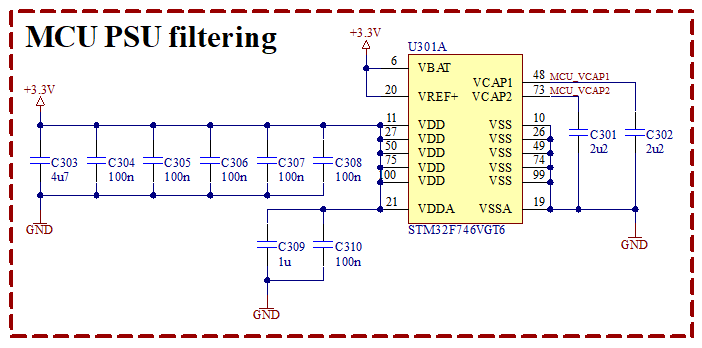
\includegraphics[width=10 cm]{Figures/MCU_02.png}
    \caption{Električna shema napajanja mikrokontrolera}
    \label{slk:MCU_PS}
\end{figure}

Električna shema napajanja napravljena je prema uputama proizvođača \cite{stmicroelectronics:an4661}. S obzirom da na ovoj ploči nema analognih signala, nije potrebno raditi analogno-digitalnu pretvorbu pa su stezaljke za napajanje analognog dijela mikrokontrolera spojene sa stezaljkama za napajanje digitalnog dijela. Također, nije potrebna precizna naponska referenca, a baterijskim napajanjem će upravljati vanjski integrirani sklop pa su te dvije stezaljke spojene na napajanje od +3,3 V.
\begin{figure}[H]
    \centering
    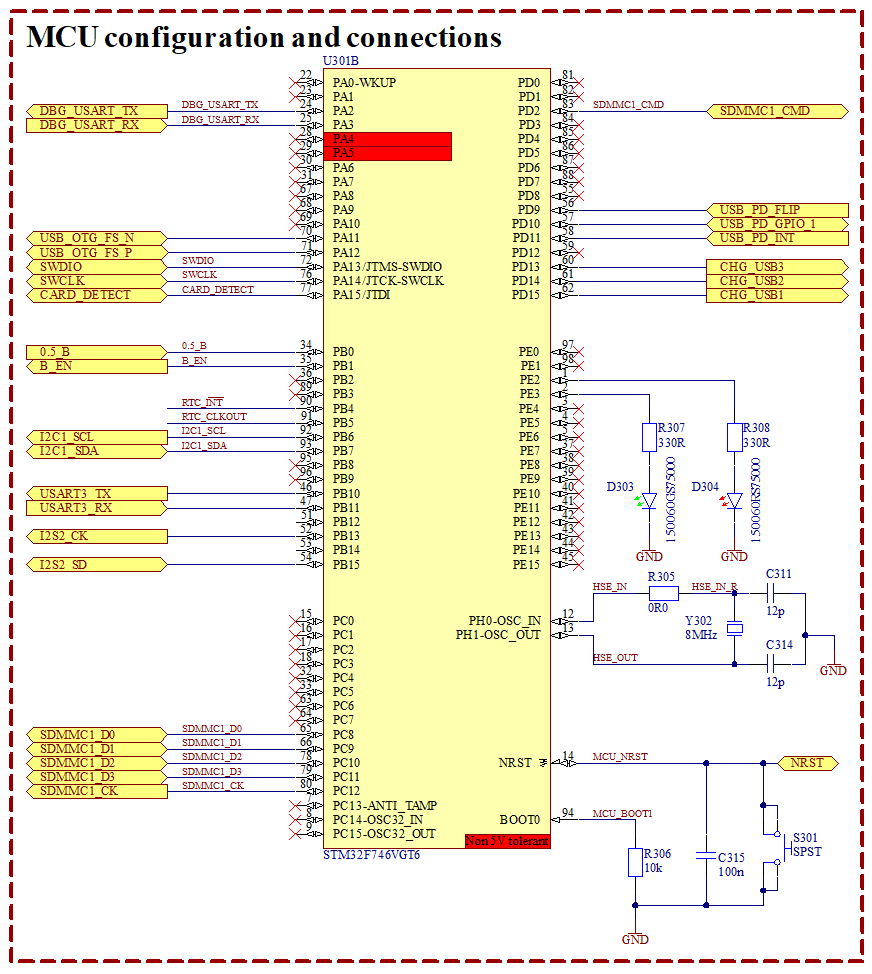
\includegraphics[width=\textwidth]{Figures/MCU_01.png}
    \caption{Električna shema periferije mikrokontrolera}
    \label{slk:MCU_PE}
\end{figure}
Postavljene su dvije svjetleće diode za pomoć pri programiranju i tipka za reset mikrokontrolera. Kod određivanja potrebnih priključaka za referencu je korišteno razvojno okruženje STM32CubeIDE. Dizajn oscilatora opisan je u priručniku proizvođača STMicroelectronics \cite{stmicroelectronics:an2867}. Oscilator koji mikrokontroler koristi je Pierceov oscilator (slika \ref{slk:PIERCE}).
\begin{figure}[hbt]
    \centering
    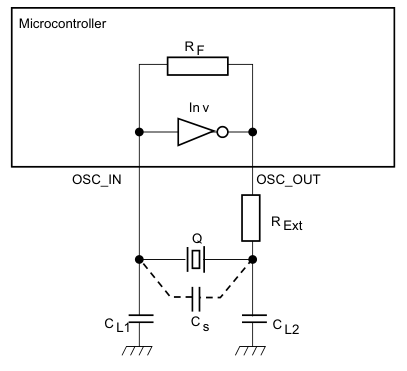
\includegraphics[width=10cm]{Figures/pierce.PNG}
    \caption{Električna shema Piercovog oscilatora \cite{stmicroelectronics:an2867}}
    \label{slk:PIERCE}
\end{figure}

\subsection{Pierceov oscilator}
Pierceov oscilator se sastoji od invertera \textit{Inv}, koji radi kao pojačalo, kristala \textit{Q}, otpornika u povratnoj vezi \textit{R\textsubscript{F}}, vanjskog otpornika za ograničenje izlazne struje invertera \textit{R\textsubscript{Ext}}, vanjskog opteretnog kapaciteta \textit{C\textsubscript{L1}} i \textit{C\textsubscript{L2}}, parazitskog kapaciteta tiskane pločice i kapaciteta između stezaljki mikrokontrolera \textit{C\textsubscript{s}}.

Uloga otpornika \textit{R\textsubscript{F}} je da inverter dovede u način rada kada se ponaša poput pojačala. Otpornik povratne veze je spojen između izlaza i ulaza pojačala čime se ulaz i izlaz drže na istom naponu i osigurava se da pojačalo radi u linearnom području rada. Ovaj otpornik je integriran u mikrokontroleru zajedno s pojačalom.

Opteretni kapacitet je ukupni kapacitet povratne veze oscilatora i mora biti jednak je kapacitetu između stezaljki kristala kako bi oscilator prooscilirao. Opteretni kapacitet specificira proizvođač kristala i označava se s \textit{C\textsubscript{L}}. Vanjskim kondenzatorima \textit{C\textsubscript{L1}} i \textit{C\textsubscript{L2}} se postavlja opteretni kapacitet povratne veze kako bi odgovarao opteretnom kapacitetu kristala. Opteretni kapacitet se računa prema sljedećoj jednadžbi:
\begin{equation} \label{eq:CLOAD}
    C_L=\frac{C_{L1}\cdot C_{L2}}{C_{L1}+C_{L2}}+C_s
\end{equation}

Kod dizajna oscilatora potrebno je izračunati kritično pojačanje petlje:
\begin{equation} \label{eq:GMCRIT}
    g_{mcrit}=4\cdot ESR \cdot {(2\pi f)}^2\cdot {(C_0 + C_L)}^2
\end{equation}
gdje je \textit{f} frekvencija oscilatora, \textit{ESR} serijski otpor kristala i \textit{C\textsubscript{0}} serijski kapacitet kristala. Ovaj parametar je potrebno izračunati kako bi se moglo provjeriti hoće li se oscilator upaliti i prooscilirati. Dobiveni podatak se uspoređuje sa specificiranim vrijednostima transvodljivosti \textit{g\textsubscript{m}} u dokumentaciji mikrokontrolera. Da bi oscilator proradio mora se proračunati margina pojačanja i treba vrijediti:
\begin{equation} \label{eq:GMARGIN}
    {gain}_{margin}=\frac{g_m}{g_{mcrit}}>5
\end{equation}

Kako ne bi došlo do kvara kristala potrebno je ograničiti snagu koja se na njemu disipira s pomoću vanjskog otpornika \textit{R\textsubscript{Ext}}. Maksimalna snaga koja se može disipirati na kristalu naznačena je u dokumentaciji proizvođača. Ovaj otpornik s kondenzatorom \textit{C\textsubscript{L2}} formira niskopropusni filtar kako bi oscilator proradio na osnovnoj frekvenciji, a ne na višim harmonicima. Ako snaga disipirana na kristalu bude veća od maksimalne dozvoljene, onda je vanjski otpornik obavezan i mora se proračunati, u suprotnom ga nije potrebno stavljati. Vrijednost otpornika se računa na sljedeći način:
\begin{equation} \label{eq:REXT}
    R_{Ext}=\frac{1}{2\pi f C_{L2}}
\end{equation}

\subsection{Dizajn oscilatora}

Oscilator je vidljiv na slici \ref{slk:MCU_PE}. Odabran je kristal NX8045GB proizvođača NDK. Njegove karakteristike su sljedeće:
\begin{itemize}
    \item \textit{C\textsubscript{L}} = 2 pF
    \item \textit{ESR} = 200 $\Omega$
    \item \textit{f} = 8 MHz
\end{itemize}
\textit{C\textsubscript{0}} nije naznačen pa se uzima vrijednost 0. Uzimajući za parazitni kapacitet \textit{C\textsubscript{s}} = 2 pF i koristeći formulu \ref{eq:CLOAD} dobiju se vrijednosti kondenzatora \textit{C\textsubscript{L1}} = \textit{C\textsubscript{L2}} = 12 pF. Odabir parazitnog kapaciteta je približan jer se ne može znati unaprijed bez mjerenja dovršene tiskane pločice. Kod odabira kondenzatora potrebno je obratiti pažnju na dielektrik kondenzatora i tolerancije. Kako bi frekvencija oscilatora bila što stabilnija, potrebno je koristiti temperaturno stabilan dielektrik, odnosno kondenzatore klase 1. Korišteni kondenzatori imaju C0G dielektrik. Koristeći jednadžbu \ref{eq:GMCRIT} dobiva se ${g_{mcrit} = 0,1294 \quad \textrm{mA/V}}$. Iz dokumentacije mikrokontrolera se dobiva ${g_m = 1\quad \textrm{mA/V}}$. Iz uvjeta \ref{eq:GMARGIN} dobiva se ${{gain}_{margin}=\nolinebreak 7,73}$, čime je uvjet zadovoljen. S obzirom da nije moguće odrediti koliko će se kristal grijati, za vanjski otpornik postavljen je otpornik vrijednosti 0 $\Omega$ pa u slučaju prevelike disipacije snage na kristalu moguće je na njegovo mjesto zalemiti otpornik odgovarajuće vrijednosti prema jednadžbi \ref{eq:REXT}.

\section{Sat realnog vremena (RTC)}

S obzirom da uređaj treba uskladiti podatke s mikrofona i narukvice, potrebno je precizno praćenje vremena. U tu svrhu dodan je vanjski RTC PCF8653 proizvođača NXP \cite{nxp:pcf8654}. Za ovaj integrirani sklop postoji već razvijena programska podrška u ZephyrOS operacijskom sustavu za rad u stvarnom vremenu, pa je razvoj programske potpore za uređaj znatno olakšan. Električna shema RTC-a prikazana je na slici \ref{slk:RTC}.
\begin{figure}[hbt]
    \centering
    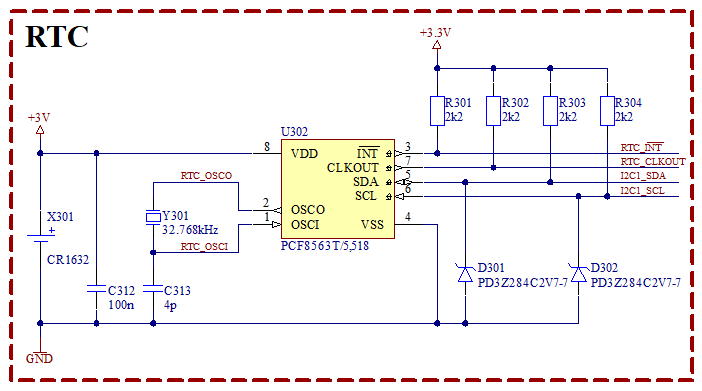
\includegraphics[width=10 cm]{Figures/RTC.png}
    \caption{Električna shema RTC-a}
    \label{slk:RTC}
\end{figure}
S obzirom da se litij-ionska baterija, koja napaja cijeli uređaj, može isprazniti, otkopčati ili na neki drugi način se može prekinuti napajanje s vanjske baterije, RTC se napaja iz litijske baterije kako praćenje vremena ne bi bilo izgubljeno. S obzirom da je napon litijske baterije 3 V, a napon ostatka sustava 3,3 V, na I\textsuperscript{2}C linije dodane su Zener diode s probojnim naponom od 2,7 V, čime se maksimalni napon ograničava kako ne bi došlo do oštećenja integriranog tijekom komunikacije s mikrokontrolerom.

\section{Bežična komunikacija}
Električna shema podsustava za bežičnu komunikaciju prikazana je na slici \ref{slk:WIFI}. Radi lakšeg razvoja odabran je razvojni sustav ESP32-C3-WROOM-02 proizvođača Espressif Systems. Električna shema je razvijena prema preporukama proizvođača \cite{espressif:wroom02}. Dodan je još jedan kratkospojnik za ispitivanje funkcionalnosti reseta sustava.
\begin{figure}[!hbt]
    \centering
    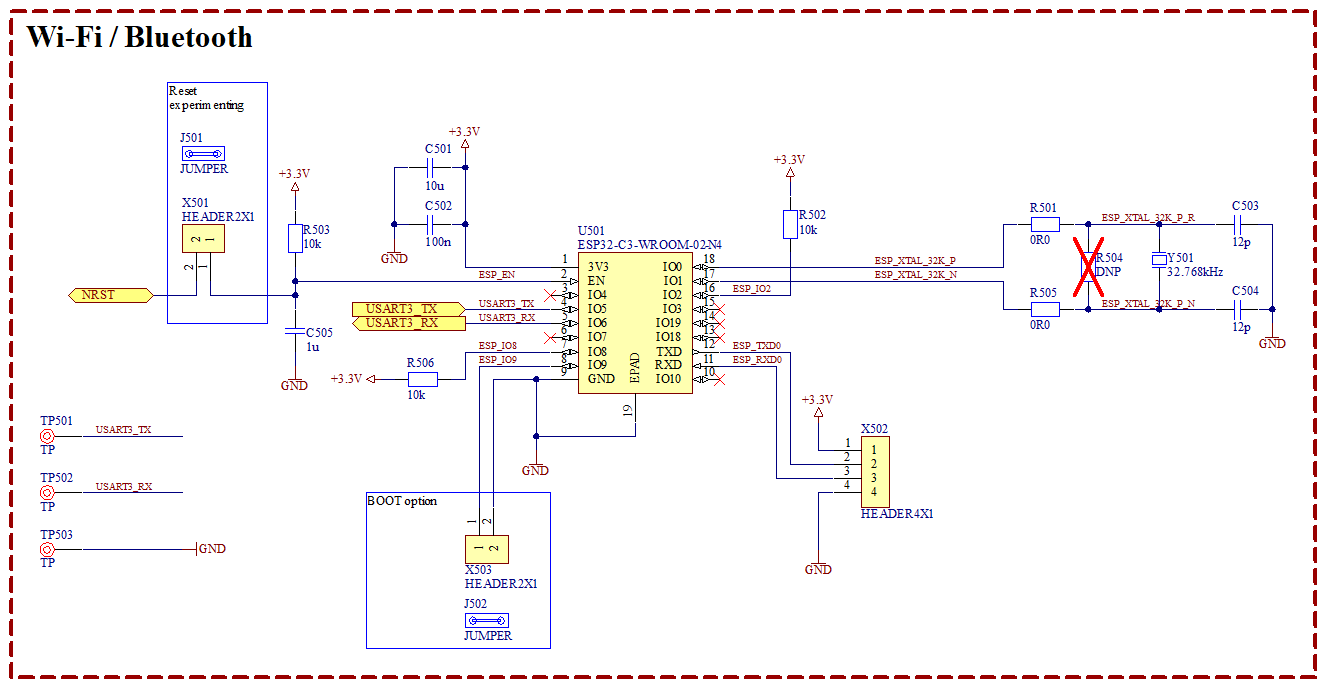
\includegraphics[width=\textwidth]{Figures/WIRELESS.png}
    \caption{Električna shema podsustava za bežičnu komunikaciju}
    \label{slk:WIFI}
\end{figure}

\section{SD kartica i konektori}
Za pohranu podataka na uređaju se nalazi SD kartica standardne veličine. Razlog odabira ove veličine jest taj da uređaj onda podržava i standardnu SD karticu i adapter za SD kartice manje veličine. Elektrčina shema SD konektora prikazana je na slici \ref{slk:SD}. Konektor ima ESD zaštitu u obliku diode D401 i filtriranje napajanja putem mreže koja se sastoji od kondenzatora i feritne perle. Na svim komunikacijskim linijama se nalaze pritezni otpornici, a linija za takt ima terminacijski otpor od 49,9 $\Omega$ kako bi se suzbila refleksija. Kako CD stezaljka za detekciju spojene kartice ne bi ostala plutajuća dodan je pritezni otpornik od 1 M$\Omega$. Razlog odabira tako velikog otpora je unutarnji pritezni otpornik prema napajanju na SD karticama pa se velikim otporom suzbija efekt naponskog djelila.
\begin{figure}[h!bt]
    \centering
    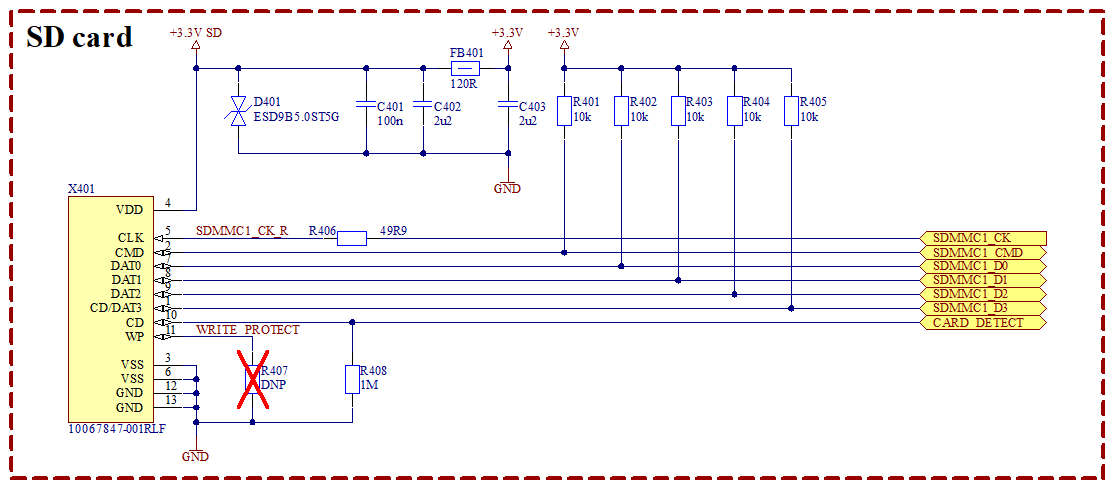
\includegraphics[width=\textwidth]{Figures/SD.png}
    \caption{Elektrčina shema konektora SD kartice}
    \label{slk:SD}
\end{figure}

Za upisivanje korisničkog programa u Flash memoriju mikrokontrolera potreban je konektor za SWO sučelje. Dodatno, za testiranje programske podrške i komunikaciju s računalom potreban je konektor za UART sučelje. Sheme konektora prikazane su na slikama \ref{slk:UART_SWO}.
\begin{figure}[!hbt]
    \centering
    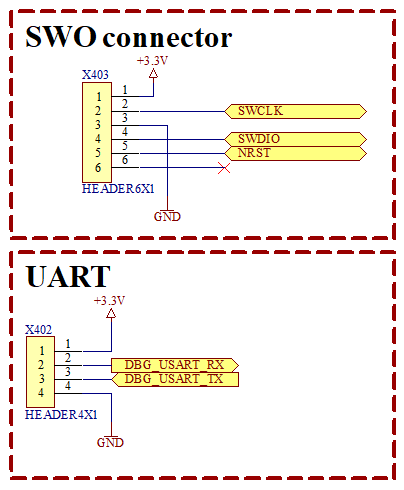
\includegraphics[width=6 cm]{Figures/SWO_UART.png}
    \caption{Elektrčina shema konektora za UART i SWO sučelje}
    \label{slk:UART_SWO}
\end{figure}

Za mikrofon se koristi evaluacijska pločica STEVAL-MIC003V1 (slika \ref{slk:STEVAL}) na kojoj se nalazi MEMS mikrofon IMP34DT05 proizvođača STMicroelectronics \cite{stmicroelectronics:steval}. Za ovaj mikrofon također postoji razvijena programska podrška unutar ZephyrOS operacijskog sustava za rad u stvarnom vremenu. Ove evaluacijske pločice na sebi imaju montirane muške konektore s razmakom od 7 mm, pa se ovdje koriste ženski konektori (slika \ref{slk:MEMS}).
\begin{figure}[h!bt]
    \centering
    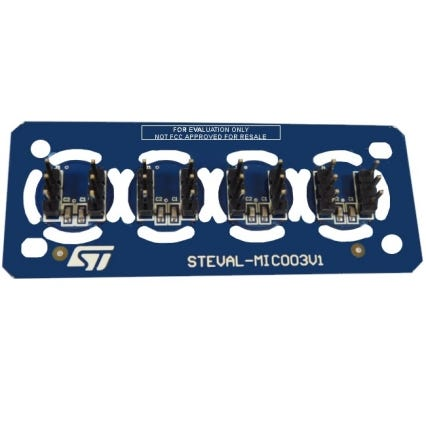
\includegraphics[width=6 cm]{Figures/STEVAL.jpg}
    \caption{STEVAL-MIC003V1}
    \label{slk:STEVAL}
\end{figure}
\begin{figure}[h!bt]
    \centering
    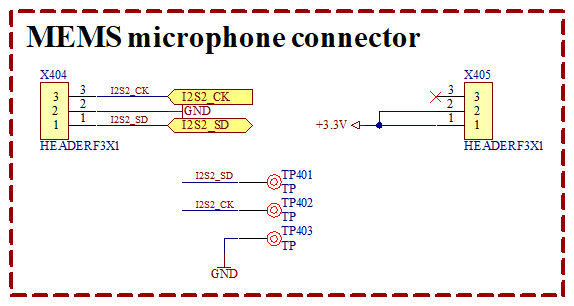
\includegraphics[width=6 cm]{Figures/MEMS.png}
    \caption{Konektori za MEMS}
    \label{slk:MEMS}
\end{figure}
Kraj konektora su postavljene testne točke za promatranje signala putem logičkog analizatora u slučaju da postoje poteškoće tijekom programiranja ili rada.

\section{Napajanje}
Nakon što su odabrane sve potrebne komponente za postizanje pune funkcionalnosti sustava, moglo se projektirati i prikladno napajanje. Prvo je bilo potrebno proračunati potrošnju sustava, a potom odabrati komponente napajanja koje mogu zadovoljiti traženu potrošnju sustava na što efikasniji način.

\subsection{Proračun potrošnje}
Napravljena je tablica potrošnje za sustave koji se napajaju s 3,3 V (tablica \ref{tab:MB3V3}). Za maksimalne i minimalne vrijednosti potrošnje uzeti su podaci iz dokumentacije komponenata, a prosječna potrošnja procjenjena je približno jer je nemoguće znati prosječnu potrošnju bez mjerenja u stvarnim uvjetima rada.
\begin{table}[htbp]
    \centering
    \caption{Potrošnja struje za sustave koji se napajaju sa 3,3 V}
    \begin{tabular}{lccc} \hline
           & Min. [mA] & Avg. [mA] & Max. [mA] \\
      MCU  & 0,00 & 60,00 & 320,00 \\
      RTC  & 0,00 & 0,80 & 50,00 \\
      SD Card & 1,25 & 25,00 & 100,00 \\
      MEMS & 0,00 & 0,65 & 10,00 \\
      Wireless & 13,00 & 82,00 & 350,00 \\ \hline
      Total on SYS & 14,25 & 168,45 & 830,00 \\ \hline
    \end{tabular}%
    \label{tab:MB3V3}%
\end{table}%
Na temelju ovih podataka se može odrediti za koliku snagu napajanje mora biti projektirano. Maksimalna struja je manja od 1 A, a uređaj nikada neće dostići toliku razinu potrošnje jer se neće koristiti sve mogućnosti najvećih potrošača (mikrokontroler i bežična komunikacija). S obzirom da korisnik neće cijelo vrijeme pričati sustav će ući u mirovanje, a prosječna struja će onda biti još manja. Imajući na umu sve navedeno, procjenjuje se da će baterija od kapaciteta 2 Ah biti dovoljna. Tek nakon ove analize mogle su biti odabrane sve prikladne komponente za napajanje.

\subsection{Baterija i punjač baterije}
Za punjač baterije odabran je BQ24166 proizvođača Texas Instruments (slika \ref{slk:BQ24166}). Ovaj integrirani sklop u sebi ima integriran sustav za upravljanje tokom snage \cite{ti:bq24166}. BQ24166 se može napajati s dva ulaza, ulaza za USB ili ulaza za druge vrste napajanja (AC/DC adapter, DC laboratorijski izvor napajanja, itd.), a da pritom u isto vrijeme puni bateriju i na svom izlazu daje napon baterije, s tim da izlazni napon neće pasti ispod 3,5 V. U tu svrhu u integrirani sklop je ugrađen silazni prekidački regulator napona, kako bi se kod punjenja baterije konstantnim naponom dobio izlazni napon od 4,2 V potreban za punjenje. Ako na ulaz integriranog sklopa nije spojeno ništa, onda se na izlaz izravno prosljeđuje napon baterije. U slučaju da napon baterije padne ispod 3,5 V, a da pritom ništa nije spojeno na ulaz integriranog sklopa, izlazni napon se regulira na 3,5 V, čime se baterija može u potpunosti iskoristiti. Ovaj integrirani sklop također ima ugrađene zaštite od prenapona, a jednim otpornikom moguće je i programirati prekostrujnu zaštitu. Također je jednim otpornikom moguće i programirati maksimalnu struju punjenja baterije.
\begin{figure}[!hbtp]
    \centering
    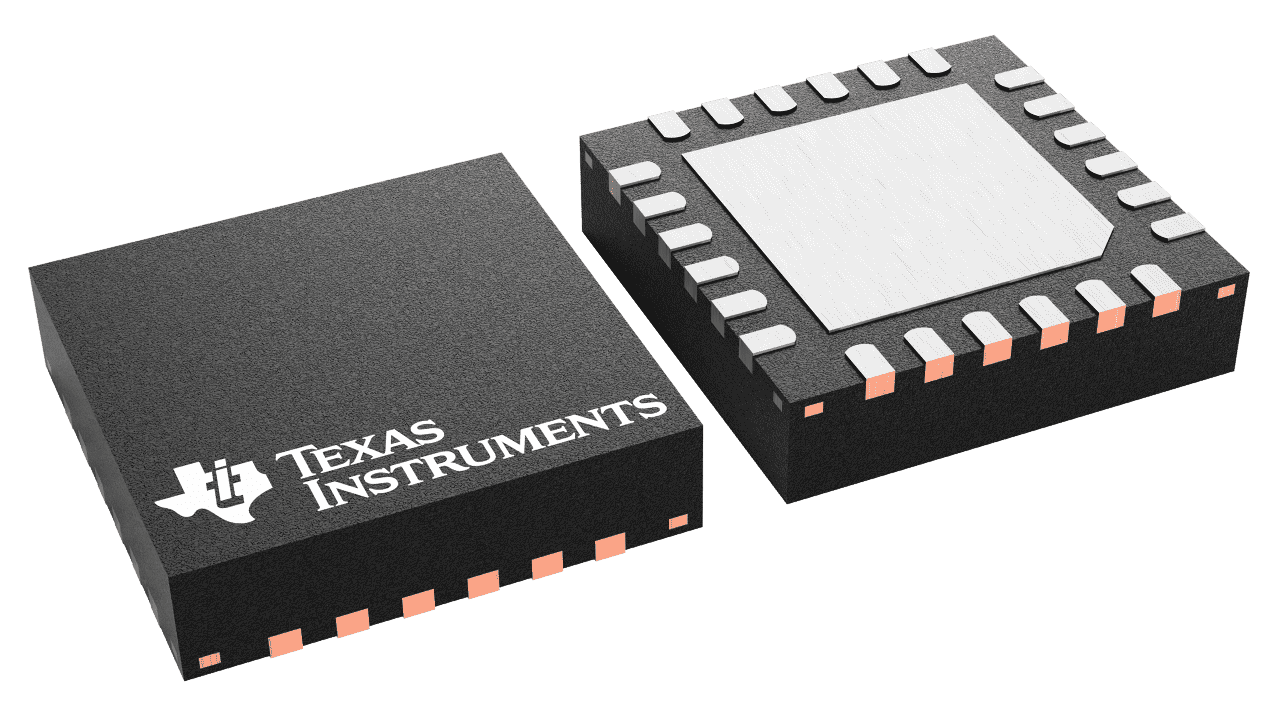
\includegraphics[width = 6 cm]{Figures/bq24166.png}
    \caption{BQ24166 u QFN kućištu}
    \label{slk:BQ24166}
\end{figure}

Elektrčina shema baterijskog punjača prikazana je na slici \ref{slk:MB_BATCHG}. Blokadni kondenzatori su postavljeni prema uputama proizvođača, a potrebno je bilo odabrati odgovarajuće otpornike za programiranje prekostrujne zaštite i maksimalne struje punjenja, kao i prikladnu zavojnicu. Kako bi se navedene komponente odabrale na odgovarajući način, potrebno je znati izlaznu struju iz punjača.
\begin{figure}[!htb]
    \centering
    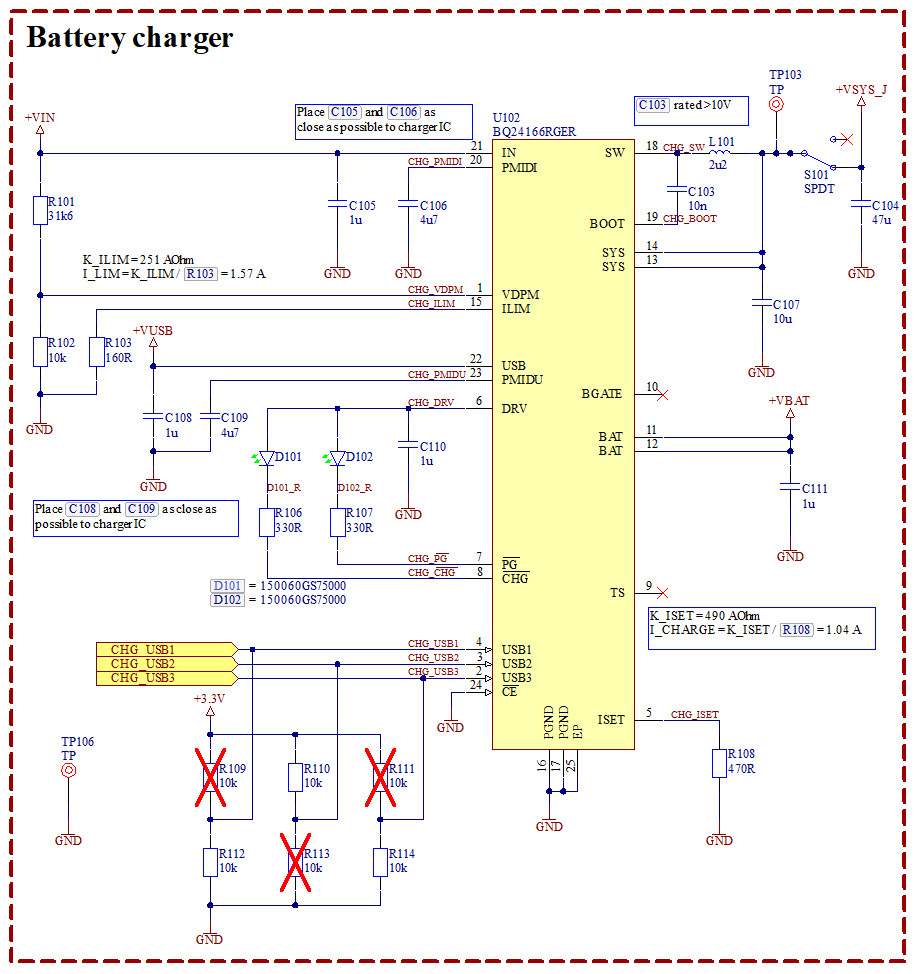
\includegraphics[width = \textwidth]{Figures/MB_BATCHG.png}
    \caption{Električna shema baterijskog punjača}
    \label{slk:MB_BATCHG}
\end{figure}

Na izlazu punjača se nalazi linearni regulator napona s niskim padom napona (190 mV na struji od 1,5 A) koji regulira napon na 3,3 V (slika \ref{slk:MB_LDO}). Imajući na umu da je ulazna struja linearnog regulatora otprilike ista kao i izlazna struja, dobiva se izlazna struja baterijskog punjača, što odgavara proračunu iz tablice \ref{tab:MB3V3}, a to je ujedno i struja koju daje baterija. Proizvođač preporuča zavojnice vrijednosti 2,2 $\mu$H za slučaj manje valovitosti struje i manjeg ograničenja na prostor i 1,5 $\mu$H u slučaju manjeg ograničenja na valovitost i većeg ograničenja na prostor. Ovdje je odabrana vrijednost od 2,2 $\mu$H, a zavojnica je odabrana tako da su struje zasićenja zavojnice i maksimalna struja koju zavojnica može podnijeti veće od dvostruke izlazne struje, što je slučaj najveće valovitosti.
\begin{table}[!htb]
    \centering
    \caption{Ograničenja struje USB-a \cite{ti:bq24166}}
    \begin{tabular}{|c|c|c|c|c|} \hline
    IUSB3 & IUSB2 & IUSB1 & Ograničenje ulazne struje & Minimalni napon \\
    \hline
    0 & 0 & 0 & 100 mA & 4,28 V \\
    \hline
    0 & 0 & 1 & 500 mA & 4,44 V \\
    \hline
    0 & 1 & 0 & 1,5 A & 4,44 V \\
    \hline
    0 & 1 & 1 & Visoka impedancija & Nikakav \\
    \hline
    1 & 0 & 0 & 150 mA & 4,28 V \\
    \hline
    1 & 0 & 1 & 900 mA & 4,44 V \\
    \hline
    1 & 1 & 0 & 800 mA & 4,44 V \\
    \hline
    1 & 1 & 1 & Visoka impedancija & Nikakav \\
    \hline
    \end{tabular}%
    \label{tab:USB_ILIM}%
\end{table}%

Radi potreba testiranja dodani su pritezni otpornici na stezaljkama USB1, USB2 i USB3. Ovisno o logičkim razinama na tim stezaljkama moguće je ograničiti struju na ulazu za USB. Razne konfiguracije ograničenja struje prikazane su u tablici \ref{tab:USB_ILIM}. Uobičajeno ograničenje u ovom slučaju je 1,5 A.

Da bi se dobila maksimalna ulazna struja punjača potrebno je uzeti u obzir najgori mogući slučaj: baterija je odspojena, potrošnja sustava je maksimalna. Unutar punjača se nalazi silazni pretvarač, dakle vrijedi:
\begin{equation}
    P_{IZ}=\eta \cdot P_{UL}
\end{equation}
\begin{equation} \label{eq:BUCK}
    U_{IZ}\cdot I_{IZ}=\eta \cdot U_{UL} \cdot I_{UL}
\end{equation}
gdje je \textit{U\textsubscript{IZ}} i \textit{I\textsubscript{IZ}} izlazni napon, odnosno struja, \textit{U\textsubscript{UL}} i \textit{I\textsubscript{UL}}, ulazni napon, odnosno struja, a $\eta$ učinkovitost. Provjerom dokumentacije proizvođača, može se uzeti efikasnost od 90 \% (slika \ref{slk:EFFICIENCY}).
\begin{figure}[H]
    \centering
    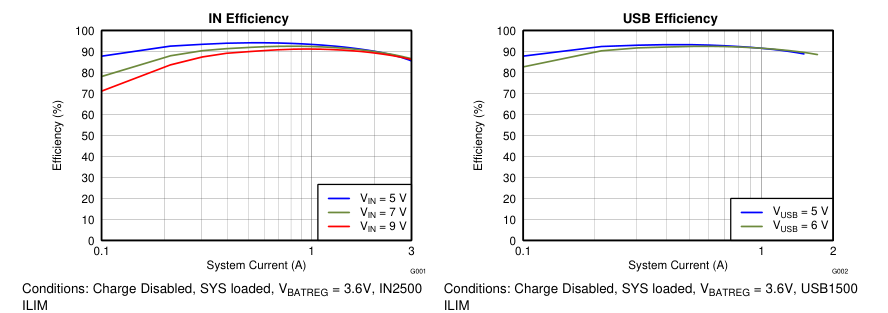
\includegraphics[width=\textwidth]{Figures/EFFICIENCY.PNG}
    \caption{Ovisnost efikasnosti o izlaznoj struji punjača \cite{ti:bq24166}}
    \label{slk:EFFICIENCY}
\end{figure}
\noindent Iz jednadžbe \ref{eq:BUCK} se sada može dobiti izraz za ulaznu struju:
\begin{equation} \label{eq:IN_CURR}
    I_{UL}=\frac{\eta \cdot U_{IZ} \cdot I_{IZ}}{U_{UL}}
\end{equation}
Iz jednadžbe \ref{eq:IN_CURR} je vidljivo da će ulazna struja biti najveća kada je ulazni napon što manji, što u ovom slučaju iznosi 5 V. Za izlazni napon se također uzima najgori slučaj od 4,2 V. Sada se za maksimalnu ulaznu struju punjača uz odspojenu bateriju dobiva iznos od ${I_{UL,BATOFF} = 627,48\textrm{ mA}}$.
\begin{figure}[H]
    \centering
    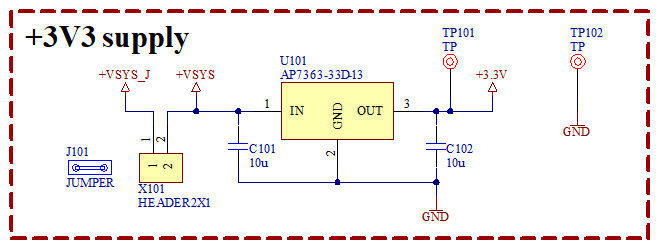
\includegraphics[width = 10 cm]{Figures/MB_LDO.png}
    \caption{Linearni regulator napona}
    \label{slk:MB_LDO}
\end{figure}

Imajući na umu da će do maksimalne potrošnje doći rijetko, ako uopće, i činjenicu da će sustav imati mogućnost ulaska u način rada mirovanja, može se uzeti kapacitet baterije od 2 Ah, čime se postiže balans trajanja baterije i cijene. U tom slučaju dovoljno je ograničiti punjenje baterije na 1 A, a izračun otpornika je vidljiv na shemi (slika \ref{slk:MB_BATCHG}). Odgovarajuće konstante za izračun otpornika su dobivene iz dokumentacije proizvođača. Sada je isto pomoću jednadžbe \ref{eq:IN_CURR} moguće izračunati ulaznu struju; ${I_{UL,BATCHG} = 756\textrm{ mA}}$. Ukupna maksimalna ulazna struja je stoga:
\begin{equation}
    I_{UL,MAX}=I_{UL,BATCHG}+I_{UL,BATOFF} = 1.38\textrm{ A}
    \label{eq:IN_CURR_MAX}
\end{equation}
Uz dodatak sigurnosne zalihosti, za prekostrujnu zaštitu se uzima 1,5 A. Za potrebe testiranja i otklanjanje evenutalnih grešaka na ulaz linearnog regulatora dodan je kratkospojnik.

\subsection{Baterijska zaštita}
S obzirom na mnoge opasnosti vezane uz korištenje litij-ionskih baterija, potrebno je dizajnirati prikladnu zaštitu za bateriju. U tu svrhu odabran je BQ29700 proizvođača Texas Instruments, prikazan na slici \ref{slk:BQ29700}. Ovaj integrirani sklop ima zaštitu baterije od preniskog i previsokog napona, prejake struje pražnjenja i punjenja te kratkog spoja. Električna shema sklopa za zaštitu baterije prikazana je na slici \ref{slk:MB_BATPROT}.
\begin{figure}[hbt]
    \centering
    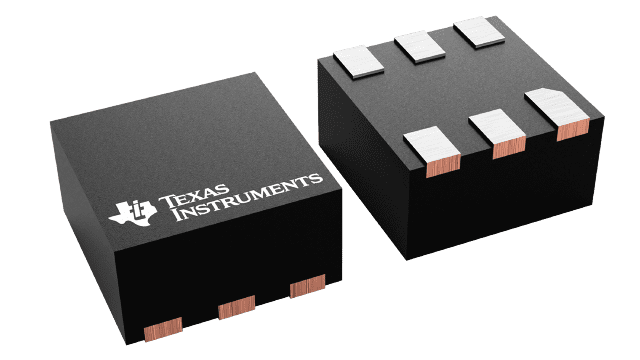
\includegraphics[width=6 cm]{Figures/BQ29700.png}
    \caption{BQ29700}
    \label{slk:BQ29700}
\end{figure}
\begin{figure}[!hbt]
    \centering
    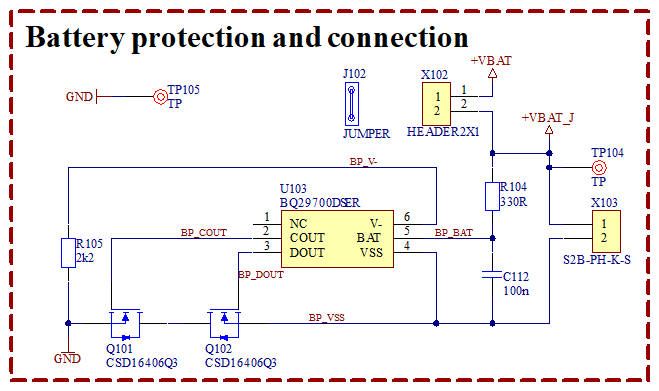
\includegraphics[width=10 cm]{Figures/MB_BATPROT.png}
    \caption{Elektrčina shema sklopa za zaštitu baterije}
    \label{slk:MB_BATPROT}
\end{figure}
Otpornici i kondenzatori su odabrani prema preporukama proizvođača, dok se tranzistori biraju prema potrebama sustava tijekom dizajna \cite{ti:bq29700}. Napon baterije se mjeri putem BAT i VSS stezaljki integriranog sklopa. U slučaju previsokog napona isključuje se tranzistor Q101, a u slučaju preniskog napona isključuje se tranzistor Q102. Struja se mjeri putem stezaljki V- i VSS, dakle putem otpora tranzistora Q101 i Q102. U slučaju prevelike struje pražnjenja ili kratkog spoja isključuje se tranzistor Q102, a u slučaju prevelike struje punjenja isključuje se tranzistor Q101.

\begin{table}[htbp]
    \centering
    \caption{Pragovi aktiviranja zaštite za bateriju \cite{ti:bq29700}}
    \begin{tabular}{|l|p{1.5cm}|p{1.5cm}|p{2.5cm}|p{2.5cm}|p{2.5cm}|} \hline
    \raggedright
    & Previsok napon & Prenizak napon & Previsoka struja punjenja & Previsoka struja pražnjenja & Struja kratkog spoja \\
    \hline
    Prag [V] & 4,275 & 2,800 & -0,100 & 0,100 & 0,5 \\
    \hline
    \end{tabular}%
    \label{tab:BQ29700}%
\end{table}%
U tablici \ref{tab:BQ29700} navedeni su pragovi napona na kojima se aktivira zaštita baterije. Ako su oba tranzistora jednaka, onda za struju kroz tranzistor vrijedi:
\begin{equation} \label{eq:TRANCUR}
    I_Q = \frac{U_{TH}}{2\cdot R_{DS(on)}}
\end{equation}
gdje je \textit{U\textsubscript{TH}} napon praga, a \textit{R\textsubscript{DS(on)}} otpor jednog tranzistora. U dokumentaciji proizvođača navodi se da tranzistor mora podržavati napon između upravljače elektrode i uvoda u iznosu od $U_{GS}=3,5\textrm{ V}$. Iz grafa ovisnosti \textit{R\textsubscript{DS(on)}} o \textit{U\textsubscript{GS}} prikazanog na slici \ref{slk:RDS_OLD} može se isčitati vrijednost otpora od $R_{DS(on)}=7,5\textrm{ m}\Omega$.
\begin{figure}[!hbt]
    \centering
    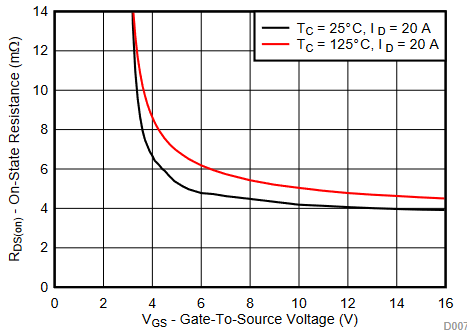
\includegraphics[width=10 cm]{Figures/RDS_OLD.PNG}
    \caption{Graf ovisnosti otpora o naponu između upravljačke elektrode i uvoda tranzistora CSD16406Q3 \cite{ti:csd1640}}
    \label{slk:RDS_OLD}
\end{figure}
\\~\\ Zaštita baterije će se aktivirati u sljedećim uvjetima:
\begin{itemize}
    \item previsoka struja punjenja $I_{OCC}=6,67\textrm{ A}$,
    \item previsoka struja pražnjenja $I_{OCD}=6,67\textrm{ A}$,
    \item struja kratkog spoja $I_{SCD}=33,33\textrm{ A}$.
\end{itemize}
Ovo je dizajn napravljen po uzoru na dokumentaciju proizvođača, u kojoj je naveden primjer za dizajn zaštite s parametrima navedenim i tablici \ref{tab:example}. Ovaj dizajn je preuzet radi užurbanog procesa dizajna, kako bi se što prije mogao dobiti prototip za ispitivanje programske podrške.
\begin{table}[htbp]
    \centering
    \caption{Parametri dizajna iz dokumentacije proizvođača \cite{ti:bq29700}}
    \begin{tabular}{|l|c|}
        \hline
        Parametar & Vrijednost \\
        \hline
        Raspon ulaznog napona & 4,5 V do 7 V \\
        \hline
        Maksimalna struja pražnjenja & 7 A \\
        \hline
        Maksimalna struja punjenja & 4,5 A \\
        \hline
    \end{tabular}
    \label{tab:example}
\end{table}
Očito je da je ovaj tranzistor loš odabir za ovaj slučaj. Pragovi struja na kojima će se zaštita aktivirati su previsoki i može doći do oštećenja sklopovlja ili baterije dogodi li se situacija kada zaštita mora proraditi. Ispravan način proračuna i odabira tranzistora bit će demonstriran u poglavlju vezanom uz izradu narukvice.

\section{USB napajanje}

S novim inačicama USB sučelja povećavala se snaga koju je USB port kao izvor napajanja mogao dati. Tablica \ref{tab:USB} prikazuje snage koje razne verzije USB sučelja mogu dati.
\begin{table}[htbp]
    \centering
    \caption{Maksimalni naponi, struje i snage raznih verzija USB sučelja \cite{ti:usb}}
    \begin{tabular}{|l|c|c|c|} \hline
    Verzija & Maksimalni napon & Maksimalna struja & Maksimalna snaga \\
    \hline
    USB 2.0 & 5 V & 500 mA & 2,5 W \\
    \hline
    USB 3.0 i USB 3.1 & 5 V & 900 mA & 4,5 W \\
    \hline
    USB BC 1.2 & 5 V & 1,5 A & 7,5 W \\
    \hline
    USB Type-C 1.2 & 5 V & 3 A & 15 W \\
    \hline
    USB PD 3.0 & 20 V & 5 A & 100 W \\
    \hline
    \end{tabular}
    \label{tab:USB}
\end{table}
Korisnik obično ne vodi računa na koju verziju sučelja spaja svoj uređaj, moguće je spojiti uređaj na USB 2.0 ili USB PD 3.0. Primjerice, ako je uređaju potrebno 1,5 A struje, a spojen je na USB 2.0, može doći do kvara izvora ili neispravnog rada uređaja. Iz tog razloga USB C priključak sadržava konfiguracijske kanale, odnosno CC linije \engl{Configuration Channels}, putem kojih uređaj i izvor mogu razmijeniti podatak o potrebnoj snazi. Način na koji CC linije funkcioniraju je prikazan na slici \ref{slk:USB_CC_LINES}. Izvor sadržava pritezne otpornike na napajanje spojene na CC linije, dok uređaj, odnosno ponor, na CC linije ima spojene pritezne otpornike na masu. Uređaj promatra CC linije kako bi zaključio kako je kabel orijentiran, dok izvor promatra napon na CC linijama, odnosno na naponskom djelilu. Mjereći napon izvor može zaključiti koliku snagu traži uređaj. Dakle, najjednostavniji način za USB napajanje uređaja je spojiti par priteznih otpornika na masu, čime se traži fiksna vrijednost snage. Međutim, uređaj koji se izrađuje u ovom radu mora imati sposobnost napajanja iz više vrsta izvora te je potrebno nešto kompleksnije rješenje.
\begin{figure}[htb]
    \centering
    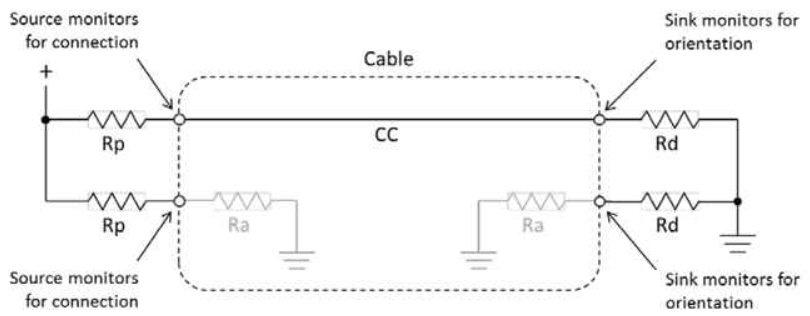
\includegraphics[width=10 cm]{Figures/USB_CC_LINES.png}
    \caption{Prikaz načina rada CC linija \cite{ti:usb}}
    \label{slk:USB_CC_LINES}
\end{figure}

Radi toga je bilo potrebno projektirati sklopovlje koje će moći zatražiti snagu od izvora, a koje će potom uključiti USB napajanje ako izvor može dati tu snagu, odnosno držati isključenim ako ne može. Postoji niz integriranih krugova koji to mogu napraviti, a za rješenje u ovom radu odabran je CYPD3177 tvrtke Cypress Technologies. Električna shema USB napajanja prikazana je na slici \ref{slk:MB_USB}. Ovaj integrirani sklop sadrži niz priteznih otpornika na stezaljkama CC1 i CC2 koje su spojene izravno na USB konektor. Struja i napon koje će integrirani sklop zahtijevati namještaju se naponskim djelilima putem priključaka ISNK\_COARSE, ISNK\_FINE, VBUS\_MIN i VBUS\_MAX. Vrijednosti otpornika na shemi odabrane su prema savjetima proizvođača \cite{ct:usb}. U ovom slučaju napon koji će se tražiti iznosi 5 V, a struja 1,5 A. Na temelju toga integrirani sklop postavlja prikladne vrijednosti otpora na CC linije. Ako izvor može dati zahtijevanu snagu, integrirani sklop postavlja stezaljku VBUS\_FET\_EN u visoku razinu, čiji je napon u visokom stanju jednak naponu koji se nalazi na USB priključku. Na taj se način uključuje vanjski P-MOSFET koji prosljeđuje napajanje s USB priključka. Otpori i kondenzatori oko tranzistora služe za usporavanje rasta napona, čime se izbjegavaju neželjene tranzijentne pojave. Za indikaciju neuspješnog dogovora između izvora i uređaja služi crvena svjetleća dioda D201. Za svrhe testiranja i otklanjanja grešaka predviđeni su kratkospojnici kojima se može odvojiti i preskočiti ovaj dio sklopovlja. U tom slučaju potrebno je zalemiti otpornike R204 i R203 u vrijednosti od 5,1 k$\Omega$, čime se traži snaga od 15 W (5 V, 3 A).
\begin{center}
    \begin{sideways}
        \begin{minipage}{1.2\linewidth}
            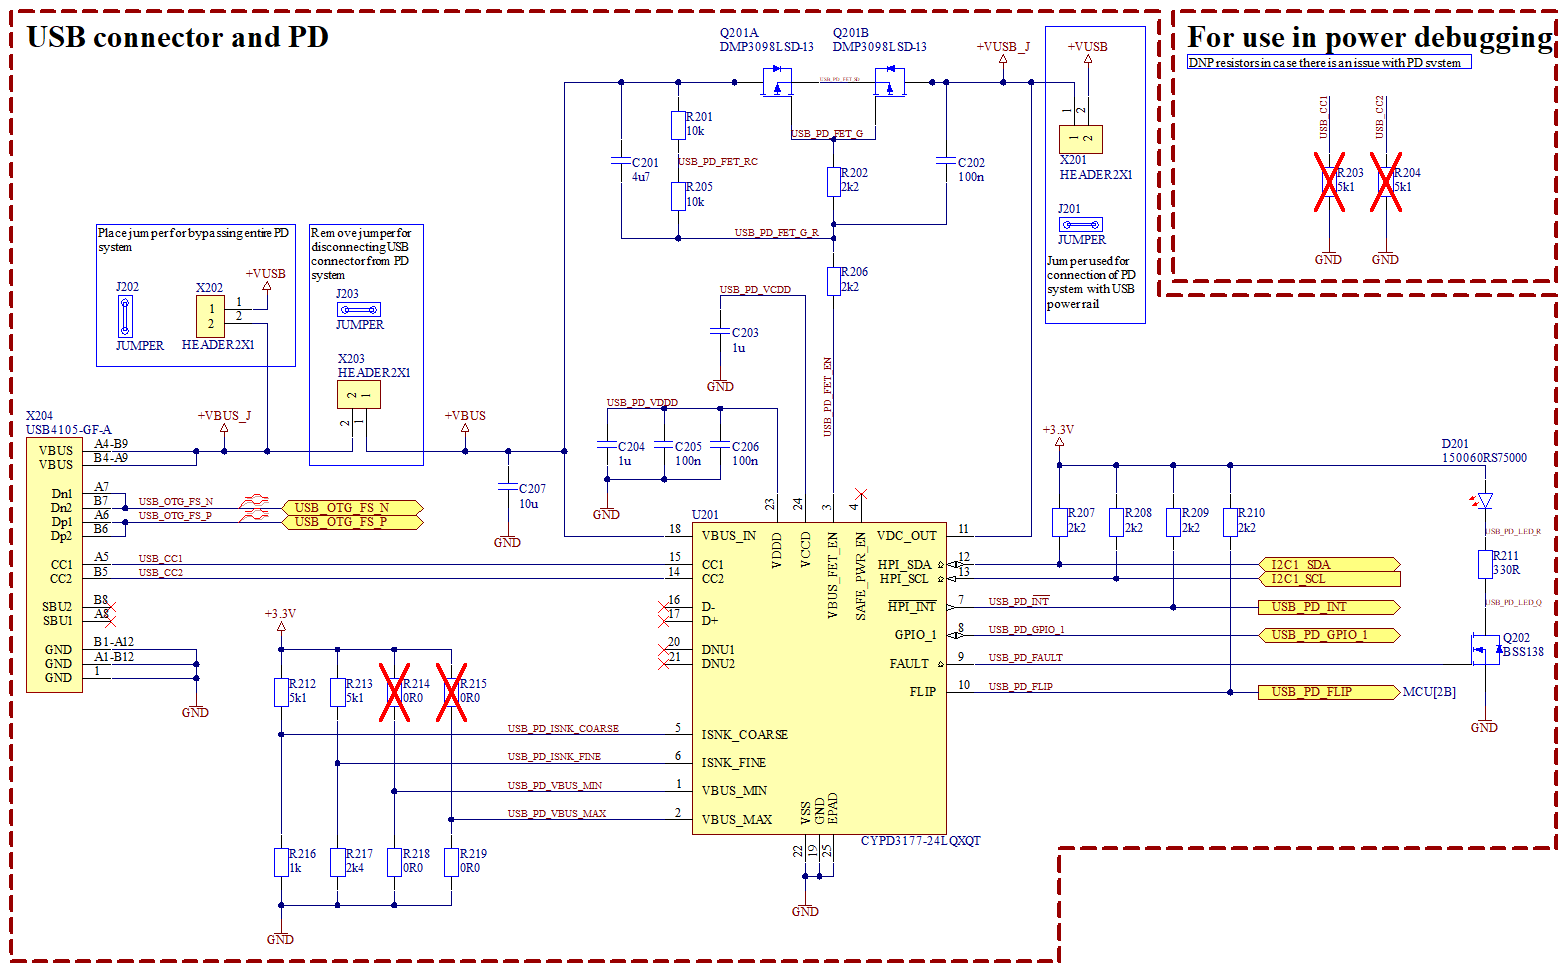
\includegraphics[width=\linewidth]{Figures/MB_USB.png}
            \captionof{figure}{Električna shema USB napajanja}
            \label{slk:MB_USB}
        \end{minipage}
    \end{sideways}
\end{center}

\section{Opis tiskane pločice}
Raspored slojeva tiskane pločice prikazan je na slici \ref{slk:MB_BOARD_STACKUP}. Oba unutarnja sloja predstavljaju ispune za uzemljenje (engl. \textit{Ground Plane}) kako bi se što bolje očuvao integritet signala na gornjem i donjem sloju. Ova konfiguracija je preuzeta s web stranice proizvođača pločice JLCPCB.
\begin{figure}[htb]
    \centering
    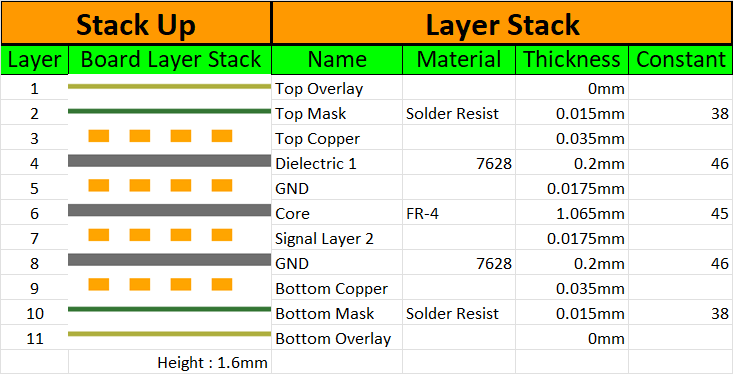
\includegraphics[width=10 cm]{Figures/MB_BOARD_STACKUP.png}
    \caption{Raspored slojeva tiskane pločice}
    \label{slk:MB_BOARD_STACKUP}
\end{figure}

Tijekom projektiranja pločice bilo je potrebno posebno obratiti pažnju na smanjenje površine komutacijske petlje kod punjača (slika \ref{slk:MB_SW_NODE}) koju čine zavojnica L101 te kondenzatori C103 i C107 (slika \ref{slk:MB_BATCHG}) kako bi se smanjile emitirane smetnje. Također je bilo potrebno obratiti pažnju na pozicioniranje antene i ravnine uzemljenja oko nje (slika \ref{slk:MB_ANTENNA}). Ovdje se može uočiti greška u projektiranju jer iako nema uzemljenja ispod antene, on se nalazi u okolini antene, što može predstavljati poteškoće u bežičnoj komunikaciji.
\begin{figure}[htb]
    \centering
    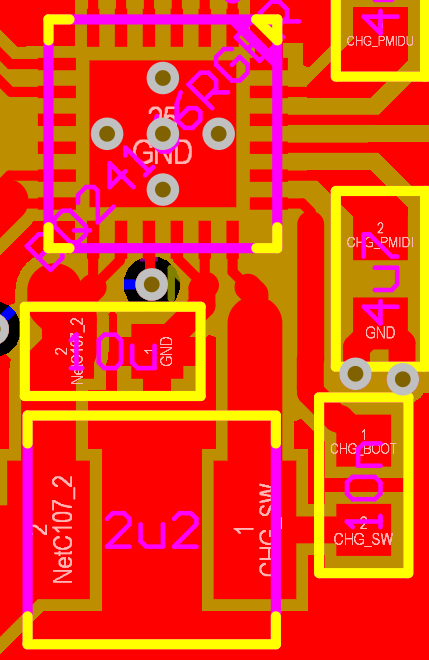
\includegraphics[width=6 cm]{Figures/MB_SW_NODE.png}
    \caption{Komutacijska petlja punjača}
    \label{slk:MB_SW_NODE}
\end{figure}
\begin{figure}[htb]
    \centering
    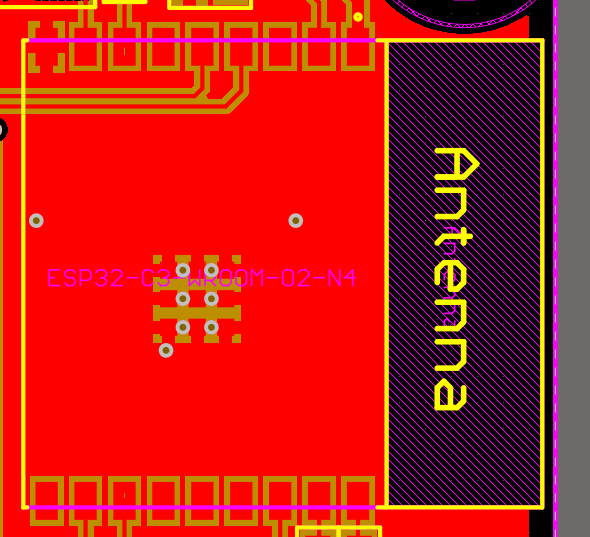
\includegraphics[width=6 cm]{Figures/MB_ANTENNA.png}
    \caption{Antena na tiskanoj pločici}
    \label{slk:MB_ANTENNA}
\end{figure}
3D prikaz projektirane tiskane pločice može se vidjeti na slici \ref{slk:MB_PCB}.
\begin{figure}[htb]
    \centering
    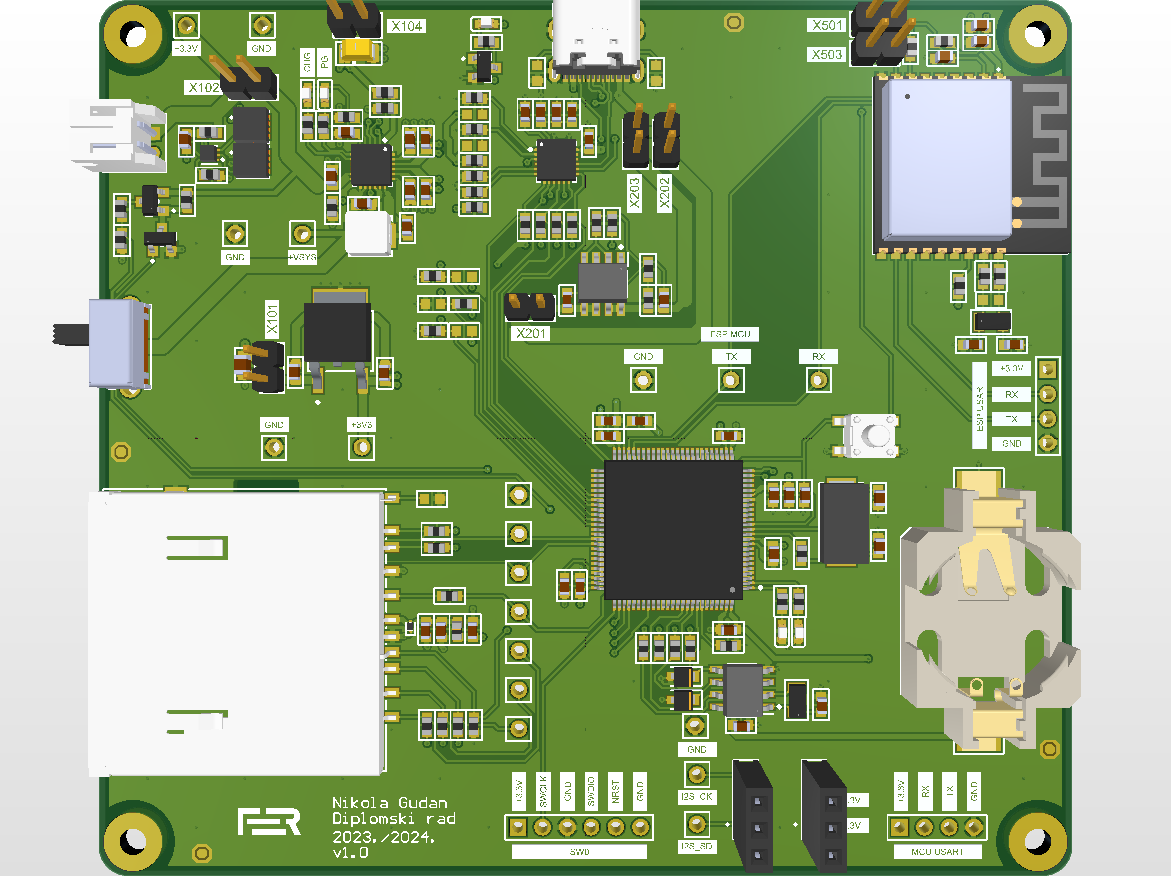
\includegraphics[width=10 cm]{Figures/MB_PCB.png}
    \caption{3D prikaz tiskane pločice}
    \label{slk:MB_PCB}
\end{figure}